\section{Runtime Example}

\toclesssubsection{Minsort}

%-------------------------------------------------------------------------------

\begin{frame}{Runtime analysis - Minsort}
  \vspace{-1em}
  \begin{figure}[!h]
    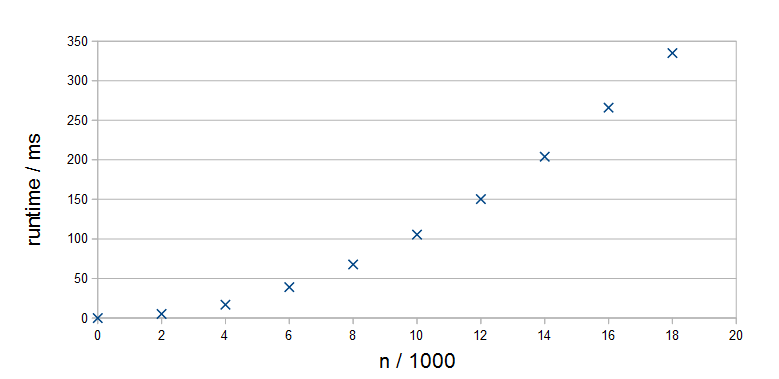
\includegraphics[width=0.75\linewidth]{Images/MinSort/Minsort.png}
    \label{fig:introduction:minsort_runtime}
  \end{figure}
  \vspace{-0.5em}
  \textbf{How long does the program run?}
  \begin{itemize}
    \item<2- |handout:1>
      In the last lecture we had a schematic
    \item<2- |handout:1>
      \textbf{Observation:} it is going to be \enquote{disproportionately} slower
      the more numbers are being sorted
    \item<3- |handout:1>
      How can we say more precisely what is happening?
  \end{itemize}
\end{frame}

%-------------------------------------------------------------------------------

\begin{frame}{Runtime analysis - Minsort}
  \textbf{How can we analyze the runtime?}
  \begin{itemize}
    \item<1- |handout:1>
      Ideally we have a formula which provides the runtime of the program for
      a specific input
    \item<2- |handout:1>
      \textbf{Problem:}
      the runtime is depends on many variables, especially:
      \begin{itemize}
        \item
          What kind of computer the code is executed on
        \item What is running in the background
        \item Which compiler is used to compile the code
      \end{itemize}
    \item<3- |handout:1>
      \textbf{Abstraction 1:}
      analyze the number of basic operations, rather than analyzing the runtime
  \end{itemize}
\end{frame}
